\chapter{Background on Metrics, Models and Management}
\label{chap:background}

Fast development of multi-core processing brings resource usage into a
cloudy world.  Performance metrics and models are prerequisites for
scientific understanding and optimization.  This chapter introduces
the area of locality analysis and optimization and reviews the
research work leading to this thesis.  It divides the material into
metrics and their measurement, metrics conversion, locality and
performance models of shared cache, and other related techniques.

% While task co-locating and cloud computing explore the potential
% synergy of resource utilization, there are many ways the performance
% is compromised due to conflicts. Either cache sharing or partitioning
% may cause performance problems.

\section{Core Metrics and Measurement}
\label{sec:bg-locality}

Locality was started as an observation that programs do not use all
their data at all times~\citep{Denning:TSE80}.  After decades of
research, it has developed into an important scientific field.  At its
foundation are locality metrics, so the concept and its effect can be
measured.  Among the basic problems are the measurement speed and
accuracy of these metrics.

\subsection{Miss Ratio and Execution Time} 
The performance of a single or a group of programs can be
observed directly.  The hardware performance counters on modern
machines enable a tool to measure program speed and count cache misses
in real-time with little costs.  However, direct observation
has difficulties in characterizing the locality cleanly due to 
dependences to the observation environment.

\begin{itemize}
\item \emph{Machine dependence.}  Different machines have different
  memory hierarchies and processors, so we cannot compare the locality
  in different programs entirely based on their performance.
\item \emph{Instrumentation dependence.}  The analysis code itself consumes
  processor and cache resources.  It may not be
  possible to completely separate the effect of the instrumentation.
\item \emph{Peer dependence.}  It is unknown how the performance
  has changed due to cache sharing.  It would have required another
  test on an unloaded system.  It is also unknown how the
  performance will change if the peer programs change.
\end{itemize}

The effect of cache on performance is often disruptive.  
Chilimbi once compared the phenomenon to ``strolling until suddenly falling over a
cliff.''\footnote{Trishul Chilimbi made this analogy in a
  presentation in 2002~\citep{ChilimbiH:PLDI02}.}  The danger is
greater in a shared environment.  As more programs are added, the
combined working set grows.  When it exceeds the size of the shared
cache, sharp performance drops would ensue.  Being peer and machine
dependent, direct testing cannot foresee a pending calamity.  Worse,
it cannot even tell whether a given parallel mix is efficient or not
without testing them individually first.

\subsection{Reuse Distance}
\label{sec:back:rd}

Instead of direct observation, off-line trace profiling can be more thorough and
can not just evaluate but also optimize a program.  % identifying causes
The most commonly used
metric is the reuse distance.  For each memory access in a
single-task execution, the reuse distance (i.e. LRU stack
distance defined by \citet{Mattson+:IBM70}) is the number of distinct data
elements accessed between this and the previous access to the same
data.  \citep{JiangZ:SIGMetrics02} also called it the inter-reference recency
(IRR).  

The reuse distance quantifies the locality of every memory access.
The locality of a program, or a loop and function inside it, is the
collection of all its reuse distances.  The collective result can be
represented as a distribution.  It is called a \emph{locality
  signature} by \citep{Zhong+:TOPLAS09} and \emph{locality profile} by
\citep{Wu+:ISCA13}.  It can be viewed as a discrete probability
density function, showing the probability of a memory access having a
certain locality.

\subsubsection{Relation with Cache Performance}

In the absence of cache sharing, the capacity miss ratio can be
written as the fraction of the reuse distance that exceeds the cache
size~\citep{Mattson+:IBM70}.  Let the test program be $A$ and cache
size be $C$, we have

\begin{equation*}
\begin{array}{l}
  P(\mbox{capacity miss by A})  = P(\mbox{A's reuse distance $>C$})
\end{array}
\end{equation*}

The reuse distance is machine independent but can give the capacity
miss ratio for cache of all sizes, as the formula shows.  More
elaborate models have been developed to estimate the miss ratio in not
just fully-associative but also direct mapped and set-associative
cache~\citep{Smith:ICSE76,HillS:TOC89,MarinM:SIGMETRICS04}.

% and for not just the tested but also all inputs of a
% program~\citep{Zhong+:TOPLAS09,Zhong+:TOC07,MarinM:SIGMETRICS04}.

\subsubsection{Miss Ratio Curve (MRC)}

The miss ratio curve (MRC) shows the miss ratio of all its cache sizes
as a discrete function.  It is easy to visualize and shows directly
the trade-off between performance and cache size.  For fully
associative LRU cache, the miss ratio curve is equivalent to the reuse
distance distribution, as the preceding formula shows.  The problem is
equivalent in theory whether it is measuring the miss ratio curve or
the reuse distance.  In practice, the miss ratio curve is defined for
only practical cache sizes, i.e. powers of two between some range,
e.g. 32KB and 8MB.  The reuse distance has the full range between 1
and the size of program data.

The full range of reuse distance represents the complete temporal
locality.  The miss ratio curve is a projection of the full
information on a subset of cache sizes.  The two would be equivalent if the
miss ratio is defined for all cache sizes between 1 and infinity.  The
unbounded size of the representation is consistent with the
theoretical result of \citet{SnirY:locality05}, who showed that
we cannot represent the temporal locality with just one or a few
numbers.  There are other metrics that represent similar information.
Chapter~\ref{chap:model} will discuss formal properties and place the
reuse distance and the miss ratio curve in relation with other
locality metrics.  In this section, we review prior work on the
measurement of the reuse distance and the miss ratio curve
together.

\subsubsection{Locality Characterization and Optimization}

% Reuse distance has found many uses in workload characterization
% and program optimization. 

Reuse distance has found many uses in workload characterization
and program optimization. The signature shows quantitatively how the
locality changes with the program input, and
the changes can be predicted as in whole-program locality analysis
\citep{Zhong+:TOPLAS09,MarinM:SIGMETRICS04,Fang+:CC06}, which is used to predict the miss ratio of all
inputs and cache sizes\citep{Zhong+:TOC07}.  The signature can be
also modeled for each memory reference and used to find critical
memory loads and important program paths, as shown by Fang et
al.~[\citeyear{Fang+:PACT05,Fang+:CC06}] \citet{MarinM:SIGMETRICS04}
models the locality signature at reference, loop, and function levels
to predict performance across different computer architectures.
Beyls and D'Hollande [\citeyear{BeylsD:HPCC06,BeylsD:CF06}] builds a
program tuning tool \emph{SLO}, which identifies the cause of long
distance reuses and gives improvement suggestions for restructuring the
code.  In addition to cache misses, reuse distance has been used to predict
cross-architecture performance (profiling on one machine and
predicting for another) \citep{MarinM:SIGMETRICS04},
response time in server systems~\citep{Kelly+:HP04}, and
usage patterns in web reference streams~\citep{Almeida+:PDIS96}. 
\citet{Zhong+:TOPLAS09} classifies these and other uses of reuse
distance as ``Five Dimensions of Locality'' and reviews the analysis
techniques for program input, code, data, execution phase and program
interaction.  

\bigskip

Reuse distance provides a common foundation to model behavior, predict
machine performance, and guide program optimization. 
Locality analysis is to summarize and decompose reuse distances.
Locality optimization is to shorten long reuse
distances.  In addition, it is free of the machine, instrumentation
and peer dependences.  The downside, however, is the complexity
of measuring reuse distance.  Next we review the existing work on
the measurement problem.

\subsubsection{Precise Measurement}
Reuse distance is one of the stack distances defined in the seminal
paper in 1970 by \citet{Mattson+:IBM70}. The stack
algorithm in the paper needed $O(nm)$ to profile a trace with $n$ accesses to $m$
distinct data.  The efficiency has been steadily improved over the
past four decades.  In 1975, \citet{BennettK:IBM75} organized
the trace as a tree and reduced the cost to $O(n \log
n)$.  In 1980, \citet{Olken:LBL81} made the
tree compact and reduced the cost further to $O(n\log m)$.  Till
today, the Olken algorithm is the most efficient asymptotic solution
for precise measurement.

There are practical improvements to the basic algorithms.  {\em Cheetah}
implemented the Olken algorithm using a
splay-tree~\citep{Sugumar:Dissertation}.  It became part of the
widely used SimpleScalar simulator~\citep{BurgerA:TR97}.
\citet{Almasi+:MSP02} used a different tree representation to further
improve the efficiency.
 
Ding and Zhong gave an approximation algorithm, first published in
2003~\citep{DingZ:PLDI03,Zhong+:TOPLAS09}.  It guarantees a relative
precision, e.g. 99\%, and takes $O( n \log \log m)$, which is
effectively linear to $n$ for any practical values of data size $m$.
Zhong et al. also gave an algorithm that guarantees a constant error
bound and does not reduce the asymptotic cost~\citep{Zhong+:LCR02}.
In an independent implementation, \citet{Schuff+:PACT10} reported that the average cost of the
$O(n \log \log m)$ method is as high as
several thousand times slowdown.

Zhong et al. gave a lower bound result showing that the space
cost of precise measurement is at least $O(n \log n)$, indicating that
reuse distance is fundamentally a harder problem than streaming, i.e. 
counting the number of 1's in a sliding window, which can be done
using $O(n)$ space~\citep{Zhong+:TOPLAS09}.  

Cache locality depends on cache management.  Reuse distance shows the
locality in the LRU cache.  For random
replacement cache, \citet{Zhou:NPC10} developed a one-pass
deterministic profiling algorithm to compute the average miss rate
(instead of simulating many times and taking the average).

% This thesis can parallelize the analysis.

\subsubsection{Approximation by Reuse Time}
While the reuse distance counts the number of distinct memory
accesses, the reuse time counts all accesses.  It is simply the difference in logical
time between the previous access and the current reuse and can be measured
quickly in $O(n)$ time.  The 
working set theory used the reuse time (inter-reference gap) to compute the time-window miss
rate~\citep{DenningS:CACM72}.  If we take time-window miss rate as an approximation of the LRU miss
rate, we may say that the working set theory is the first
approximation technique.  

Two series of more recent studies have used the reuse time
to compute the reuse distance.  The first is StatCache and StatStack
by Hagersten and his
students~\citep{BergH:ISPASS04,BergH:SIGMETRICS05,EklovH:ISPASS10,Eklov+:HiPEAC11},\footnote{Berg and
  Hagersten used the term reuse distance for what we mean by reuse
  time~\citep{BergH:ISPASS04}.}
and the second is time-based locality approximation by Shen et
al.~\citep{Shen+:POPL07,ShenS:LCPC08,Jiang+:CC10} 
While the former 
computes the average miss
rate over time range (assuming that the miss probability function does
not change over time), 
the latter calculates the reuse signature to
infer the miss rate.  Although both using statistical analysis,
the precise formulation is different.

In \citet{BergH:ISPASS04},
each access is represented by a random
variable $X_i$, which is assigned 1 if the access $i$ is a miss and 0
otherwise.  Let accesses $i,j$ be two consecutive accesses to some
data.  The reuse time is $j-i$.  Let $P(k)$ be the probability that a
cache block is replaced after $k$ misses.  The following equation
holds

$$E[X_j] = P(X_{i+1}+X_{i+2}+...+X_{j-1})$$

By solving the equation, the goal is to infer the number of cache
misses in every time window.  The problem is actually one of
all-window analysis.  The equation, however, has just $O(n)$
variables.  To produce an estimate, Berg and Hagersten assumed
constant miss rate over time and random cache replacement,\footnote{Zhou studied random cache replacement policy and gave a
one-pass deterministic trace-analysis algorithm to compute the average
miss rate (instead of simulating many times and taking the
average)~\citep{Zhou:NPC10}.} first for
private cache~\citep{BergH:ISPASS04,BergH:SIGMETRICS05} and then for
shared cache~\citep{EklovH:ISPASS10,Eklov+:HiPEAC11}.  

In \citet{Shen+:POPL07}, the key measure is the \emph{interval access
probability} $p(\Delta)$, which is the probability of a randomly chosen
datum $v$ being accessed during a time interval $\Delta$.  It
is computed from the reuse time signature $p_{{}_T}$.

\begin{equation*}
p(\Delta) = \sum_{\tau=1}^\Delta \sum_{\delta=\tau+1}^T
{1\over{N-1}}p_{{}_T}(\delta)
\label{eq:pDelta}
\end{equation*}

\noindent In the derivation, Shen et al. assumed a Bernulli process and LRU
cache replacement, first for sequential
code~\citep{Shen+:POPL07,ShenS:LCPC08} and then for multi-threaded
code~\citep{Jiang+:CC10,Jiang+:HiPEAC10}.  

To model graph algorithms, \citet{Yuan+:ICPP12} defined the notion
\emph{vertex distance} and used statistical analysis to derive the
reuse distance.  The study examines random graphs and scale-free
graphs.  It shows the dual benefits of domain-specific analysis.  On
the one hand, the structure of a graph facilitates locality analysis.
On the other hand, locality analysis reveals the relation between the
properties of a graph, e.g.  edge density, and the efficiency of its
computation.

% These methods have been evaluated experimentally for accuracy (and
% shown effective for miss rate prediction) but in theory do not
% guaranteed to be correct or have a bounded error.

By solving the all-window analysis problem, this thesis provides a
third solution.  In Chapter~\ref{chap:fp}, we will show how to
compute the average footprint using the reuse time.  In
Chapter~\ref{chap:model}, we will how to compute the reuse distance
from the footprint.  Taking together, the two steps give a new
solution of time-based approximation.  Like previous methods, the new
solution is not guaranteed correct.  However, Chapter~\ref{chap:model}
will formalize the condition under which the approximation is correct.

\subsubsection{Sampling Analysis}
Sampling is usually effective to reduce the cost of profiling.  By
choosing a low sampling rate, it may reduce the amount of profiling
work by factors in hundreds or thousands.  
In program analysis, bursty
tracing is widely used, where the execution alternates between short
sampling periods and long hibernation
periods~\citep{ArnoldR:PLDI01,HirzelC:FDDO01,ChilimbiH:PLDI02}.  During
hibernation, the execution happens in the original code and has no
analysis overhead.

Locality sampling, however, is tricker.  Locality is about the time of
data reuse, but the time is unknown until the access actually happens.
The uncertainty has two consequences.  First, the length of the
sampling period cannot be bounded if it is to cover a sampled data
reuse pair.  Second, the analyzer has to keep examining every data
access.  Complete hibernation is effectively impossible.

The problem of locality sampling is addressed by a series of studies, including the
publicly available SLO tool~\citep{BeylsD:HPCC06}, continuous program
optimization~\citep{Cascaval+:PACT05}, bursty reuse distance
sampling~\citep{ZhongC:ISMM08}, and multicore reuse distance
analysis~\citep{Schuff+:PACT10}.
Sampling can drastically reduce the cost if sampled windows 
accurately reflect the behavior of other
windows~\citep{BergH:SIGMETRICS05,EklovH:ISPASS10,Eklov+:HiPEAC11}. 

SLO is developed by \citet{BeylsD:HPCC06}.
It instruments a program to skip every $k$ accesses and take the next
address as a sample.  A bounded number of samples are kept in a sample
reservoir---hence the name reservoir sampling. To capture the reuse,
it checks each access to see if it reuses some sample data in the
reservoir.  The instrumentation code is carefully engineered in GCC to
have just two conditional statements for each memory access (one for
address and the other for counter checking).  Reservoir sampling
reduces the time overhead from 1000-fold slow-down to only a factor of
5 and the space overhead to within 250MB extra memory.  The sampling
accuracy is 90\% with 95\% confidence.  The accuracy is measured in
reuse time, not reuse distance or miss rate. 

To accurately measure reuse distance, a record must be kept to count
the number of distinct data appeared in a reuse window. \citet{ZhongC:ISMM08} developed the bursty reuse distance sampling, which divides a
program execution into sampling and hibernation
periods.  In the sampling period, the counting
uses a tree structure and costs $O(\log\log M)$ per access.  If a
reuse window extends beyond a sampling period into the subsequent
hibernation period, counting uses a hash-table, which reduces the cost
to $O(1)$ per access.  Multicore reuse distance analysis by
\citet{Schuff+:PACT10} uses a similar scheme
for analyzing multi-threaded code.  Its fast
mode improves over hibernation by omitting the hash-table access at
times when no samples are being tracked.  Both methods track
reuse distance accurately.

StatCache by \citet{BergH:SIGMETRICS05} is based on unbiased uniform
sampling.  After a data sample is selected,
StatCache puts the page under the OS protection (at page granularity)
to capture the next access to the same datum.  It uses the hardware
counters to measure the time distance till the reuse.  OS protection
is limited by the page granularity.  Two other systems, developed by
\citet{Cascaval+:PACT05} and \citet{Tam+:ASPLOS09}, used the special support on IBM processors
to trap accesses to specific data addresses.  To reduce the cost,
these methods used a small number of samples.
\citet{Cascaval+:PACT05} used
the Hellinger Affinity Kernel to infer the accuracy of
sampling.  \citet{Tam+:ASPLOS09} predicted the miss rate
curve in real time. 

\subsubsection{Parallel Analysis}
\citet{Schuff+:PACT10} combined sampling and parallel analysis for
parallel code on multicore.  In the IPDPS conference in 2012, three
groups of researchers have made the analysis of even sequential
programs many times faster with parallel algorithms.
\citet{Niu+:IPDPS12} parallelized the analysis to run on a computer
cluster, while \citet{Cui+:IPDPS12} and \citet{Gupta+:IPDPS12}
parallelized it for GPU.

\subsubsection{Compiler Analysis}
Reuse distance can be analyzed statically for scientific code.
\citet{CascavalP:ICS03} used the dependence
analysis~\citep{AllenK:Book01}, and \citet{BeylsD:JSA05} defined
\emph{reuse distance equations} and used the Omega
solver \citep{PughW:PLDI92}.  While they analyzed conventional loops,
\citet{ChauhanS:ICS10} analyzed MATLAB scripts using dependence
analysis.  Unlike profiling whose results are usually input specific,
static analysis can identify and model the effect of program
parameters.  \citet{BeylsD:JSA05} used the reuse distance equations
for cache hint insertion, in particular, conditional hints, where the
caching decision is based on program run-time parameters.  Static and
lightweight reuse analysis was used by~\citet{Shen+:ICS05} in the IBM
compiler for array regrouping and structure splitting.

\subsubsection{Discussion}

Reuse distance is a powerful tool for program analysis.  It quantifies
the locality of every program instruction.  For a single sequential
execution, the metric is composable.  For example, the composition can
happen structurally to show the locality of larger program units such
as loops, functions and the whole program, or it can happen temporally
to show program executions as (integer valued) signals.

% The reuse distance is affected by the data access of peer
% programs. To model the effect, we need a new locality metric, the footprint.

There are at least two limitations.  First, reuse distance is
insufficient to analyze program interaction.  While programs interact
at all times in the shared cache, reuse distance provides locality
information for only reuse windows, not all windows.  Second, precise reuse
distance is still costly to measure.  Despite of the advances in sampling
and parallelization, the asymptotic cost is till more than linear.
These problems will be addressed indirectly through the study of
another locality metric, the footprint.

% OSU's study on object placement

\subsection{Footprint}
\label{sec:back:fp}

Measuring footprint requires counting distinct data elements, and the
result depends on observation windows.  The problem has long been
studied in measuring various types of reuse distances as discussed
before. However, footprint measurement is a problem more difficult
than reuse distance measurement. Given a trace of length $n$, there is
only $O(n)$ reuse windows but in total $O(n^2)$ footprint windows.
This section focuses on the measurement problem, which prior work solved
by either selecting a window subset to measure or
constructing a model to approximate.

% Intuitively, the active data usage in a time window is the working
% set, a term coined by \citep{Denning:CACM68}.

\paragraph{Direct counting for subset windows} 
\citet{Agarwal+:TOCS88} counted the number of cold-start misses for all windows
starting from the beginning of a trace ({\em cumulative cold misses}).  
Cumulative cold miss, together with warm-start region 
misses, were used to evaluate cache performance degradation
caused by operation system and multiprogramming activity. 

The footprint in single-length execution windows can be computed in
linear time.  On time-shared systems, the window of concern is the
scheduling quantum.  On these systems, the cached data of one process
may be evicted by data brought in by the next process.  Thiebaut and
Stone computed what is essentially the single-window footprint by
dividing a trace by the fixed interval of CPU scheduling quantum and
taking the average amount of data access of each
quantum~\citep{ThiebautS:TOCS87}.

\citet{DingC:PPOPP08} gave a sampling solution.  At each access,
it measures the footprint of a window ending at the current access. 
The length of the measured window is chosen at random.

For an execution of length $n$, direct counting measures the footprint
in $O(n)$ windows.  If we use direct counting to estimate all-window
footprint, we have a sampling rate $O(\frac{1}{n})$.  The sampling
rate may be too low to be statistically meaningful, or it may be
sufficient in practice.  Without a solution for all-window analysis,
we would not have a way to evaluate.

\paragraph{Footprint equations}
In a parallel environment such as today's multicore systems, programs
interact continuously, and the interference happens over all-length
windows.  \citet{Suh+:ICS01} and \citet{Chandra+:HPCA05} used a
recursive equation to estimate the footprint.  As a window of size $w$
is increased to $w+1$, the change in the footprint depends on whether
the new access is a miss.  The equation is as follows.  Consider a
random window $w_t$ of size $t$ being played out on some cache of
infinite size.  As we increase $t$, the footprint increases with every
cache miss.  Let $E[w_t]$ be the expected footprint of $w_t$, and
$M(E[w_t])$ be the probability of a miss at the end of $w_t$.  For
window size $t+1$, the footprint either increments by one or stays the
same depending on whether $t+1$ access is a cache miss.

$$E[w_{t+1}] = E[w_t](1-M(E[w_t]) + (E[w_t]+1)M(E[w_t])$$ 


The term $M(E[w_t])$ requires simulating sub-traces of all size $t$
windows, which is impractical.  \citet{Suh+:ICS01} solved it as a
differential equation and made the assumption of linear window growth
when the range of window sizes under consideration is small.
\citet{Chandra+:HPCA05} computed the recursive relation bottom up.
Neither method can guarantee a bound on the accuracy, i.e. how the
estimate may deviate from the actual footprint.

In addition, their approach produces the average footprint, not the
distribution. The distribution can be important.  Considering two sets
of footprints, A and B.  One tenth of A has size $10N$ and the rest
has size 0.  All of B has size $N$.  A and B have the same average
footprint $N$ but their different distribution can lead to very
different types of cache interference. Without the all-window
footprint distribution, we cannot tell for sure average footprint is
sufficient to model cache sharing.

The past solutions on reuse distance often make similar
estimates since the reuse distance is the footprint in a reuse window.
These techniques
~\citep{BergH:SIGMETRICS05,Shen+:POPL07,ShenS:LCPC08,DingC:MSR09,Jiang+:CC10}
were mentioned in Section~\ref{sec:back:rd}.  None of them can
guarantee the precision of the estimation.

\subsection{Analytical Models}

Instead of measuring the reuse distance or footprint, a mathematical
model may be used to characterize the cache performance.  Apex-Map
uses a parameterized model and a probe program to quickly find the
model parameter for a program and a machine\citep{StrohmaierS:CCPE07}.
\citet{IbrahimS:ICPP10} compared the result of synthetic probing and
that of reuse distance profiling.  \citet{He+:IPDPS12} used a fractal
model to estimate the miss rate curve through efficient online
analysis.

There was much work earlier on analytical models for memory paging
performance.  An extensive survey can be found in
\citet{Denning:TSE80}.  One simple formula was given by
\citet{Saltzer:CACM74}, a designer of the Multics system.  He
explained that ``Although it is only occasionally that a
mathematically tractable model happens to exactly represent the
real-world situation, often an approximate model is good enough for
many engineering calculations. The challenge ... is to maintain
mathematical tractability in the face of obvious flaws and limitations
in the range of applicability and yet produce a useful result.''
Saltzer's formula has been used by \citet{Strecker:TOCS83} in cache
modeling.

Another type of analytical models is the \emph{independent reference
  model}.  Given a program with $n$ pages, and each has an independent
access probability $p$ that adds to 1, \cite{King:IFIP71} showed that
steady miss rate exists for fully associative caches managed by LFU,
LRU, and FIFO replacement policies.  Later studies gave efficient
approximation methods for LRU and FIFO
\citep{FaginP:SIAMJC78,DanT:SIGMETRICS90}.
\citet{GuD:TR930} proved a simple relation between random access and
the reuse distance distribution (which is uniform).  The method of
\citet{DanT:SIGMETRICS90} can be used to analyze a more general
case where data is divided into multiple groups and has different
(random access) probabilities.  It is a type of composable model.

\section{Metrics Conversions and Denning's Law}

Footprint is a form of working set.  The working set theory is the
scientific basis as much for memory management as it is for cache
management.  A breakthrough is a simple formula revealed by
\citet{DenningS:CACM72} that shows the relation between the
working set, which is difficult to measure, and the frequency and
interval of data reuses, which are easy to measure.  The formula
converts between two locality metrics.  Metrics conversion is at
the heart of the science of locality, because it shows that memory
behavior and performance are just different displays of the same
underlying property.

While the proof of \citet{DenningS:CACM72} depended on idealized
conditions in infinitely long executions, subsequent research has
shown that the working set theory is accurate and effective in
managing physical memory for real applications.

% In cache analysis, a key concept is the footprint, which is the
% average amount of data a program accesses in a time period.  

There are three ways to quantify the working set: as a limit
value in Denning's original paper~\citeyear{Denning:CACM68}, the time-space product
defined by \cite{DenningS:CACM78}, and the all-window footprint just
defined in Section~\ref{sec:back:fp} (initially \cite{DingC:PPOPP08}).  The
equation Denning discovered holds in all three cases.  In our 2013
paper \citep{Xiang+:ASPLOS13}, we stated it as a law of locality and named it after its
inventor: 

\newtheorem*{law}{Denning's Law of Locality}

\begin{law}
  The working set is the second-order sum of the reuse frequency, and
  conversely, the reuse frequency is the second-order difference of
  the working set.
\end{law}

We will show the formal derivation and discuss its significance in
Chapter~\ref{chap:model}.  The footprint theory in this thesis
subsumes the infinitely long case in the original working set theory
and proves Denning's law for all executions.  It gives a
theoretical explanation to the long observed effectiveness of the
working set theory in practice.

Another important formula was given by \citet{EastonF:CACM78} for the
conversion between the cold-start and warm-start miss ratios.  The
authors called it their ``recipe''.  The recipe reveals that the
(cold-start) lifetime in cache size $C$ is the sum of the inter-miss
times of the (warm) cache for sizes smaller than $C$.  They found that
their ``estimate was almost always within 10-15 percent of the
directly observed average cold-start miss ratio.''  They further
quoted the analysis of \cite{ShedlerT:SIAMJC72} as corroborating
evidence.  In these studies as in \citet{DenningS:CACM72}, a program
is assumed to be a stationary stochastic process.  In
Chapter~\ref{chap:model}, we will show the Easton-Fagin conversion as
a natural result of a systematic theory, prove its correctness for all
program executions, and evaluate the accuracy on modern computers.

\section{Locality Models of Shared Cache}
\label{sec:locality:sharing}

\subsection{Early Models}
% before 2000

There are two types of cache sharing.  The first is time-switched
cache usage between processes.  \citet{EastonF:CACM78} studied the
difference between cold-start and warm-start miss ratios and computed
the effect of task interruptions as a weighted average of expected
cold-start miss ratios.  \citet{ThiebautS:TOCS87} defined a precise
measure called the \emph{reload transient}.  For a departing process,
the reload transient is the amount of its cached data lost when it
returns after another process is run.  To compute the reload
transient, \citet{ThiebautS:TOCS87} defined \emph{cache footprint},
which is the number of data blocks a program has in cache.  Given two
programs $A,B$, the reload transient of $A$ after $B$ is the overlap
between their cache footprints.

To compute footprints and their overlap, \citet{ThiebautS:TOCS87}
assumed that a program has an equal probability accessing any cache
block.  The probability is independent and identically distributed.
The overlap is then computed from expectations of binomial
distributions.

Instead of discrete probabilistic models, \citet{Strecker:TOCS83} put
forward an intuitive notion that a program is a \emph{continuous flow}
and fills the cache at the rate that is the product of two
probabilities: the chance of a miss and the chance that the miss
results in a new location in the cache being filled.  
A differential equation was constructed since the fill rate
is the derivative of the footprint over time.  To compute
the miss ratio, \citet{Strecker:TOCS83} used an analytical formula by
\citet{Saltzer:CACM74}.  \citet{Saltzer:CACM74} computed the inter-miss
time which he called the \emph{headway} as the number of hits between successive
misses.

The second type of sharing happens between the instruction and the
data of a program.  \citet{Stone+:TOC92} investigated whether LRU
produces the optimal allocation.  Assuming that the miss rate
functions for instruction and data are continuous and differentiable,
the optimal allocation happens at the points ``when miss-rate
derivatives are equal'' \citep{ThiebautS:TOC92}.  The miss rate
functions, one for instruction and one for data, were modeled instead
of measured.  The authors showed that LRU is not optimal, but left
open a question whether there is a bound on how close LRU allocation
is to optimal allocation.  The pressure model in
Chapter~\ref{chap:model} can be used to compute the cache allocation
and therefore answer the open question for any group of programs.

As a component of the Wisconsin Wind Tunnel (WWT) project,
\citet{FalsafiW:TOMACS97} developed a performance model for cache.
They used the formulation of \citet{ThiebautS:TOCS87} but computed the
overlap using a queuing model.  In implementation, they measured the
cold-start miss rate and used a reverse mapping to estimate the
footprint.  Since WWT ran the concurrent processes of a parallel
program, the instruction code was shared between processes.  The
sharing was modeled as the shared footprint in the overall process
footprint.

\citet{FalsafiW:TOMACS97} revised the terminology of \citet{ThiebautS:TOCS87}
and redefined the \emph{footprint} as the set of unique data blocks a
program accesses.  The \emph{projection} of the footprint is the set
of data blocks that the program leaves in cache.  Viewed in another
way, the footprint is the program data in an infinite cache, and the
projection is the data in a finite cache.  It is in their sense this
thesis used the word footprint.

\subsection{Reuse Distance in Parallel Code}

Reuse distance measures the locality of a program directly and does
not rely on the assumptions that were necessary for analytical models.
In a parallel program, we have two types of reuse distance.  One
considers only the accesses of a single task, and the other considers
the interleaved accesses of all tasks.  Using the terminology of
\citet{WuY:PACT11}, we call them private reuse distance (PRD) and
concurrent reuse distance (CRD).  The new problem in analyzing the parallel
locality is the relation between PRD and CRD.

Recent work has studied several solutions.  \citet{DingC:MSR09} built
models of data sharing and thread interleaving to compose CRD.
\citet{Jiang+:CC10} tackled the composition problem using probabilistic
analysis, in particular, the interval access probability based on
\cite{Shen+:POPL07}, discussed in Section~\ref{sec:back:rd}.

Multicore reuse distance by
\citet{Schuff+:PACT10} measured CRD directly using improved algorithms
made efficient by sampling and parallelization.  For loop-based code,
Wu and Yeung gave a scaling model to predict how the reuse distance,
both PRD and CRD, changes when the work is divided by a different
number of threads~\citep{WuY:PACT11}.  These modeling techniques have
found uses in co-scheduling~\citep{Jiang+:HiPEAC10} and multicore
cache hierarchy design~\citep{WuY:MSPC12,WuY:PACT11,Wu+:ISCA13}.

\subsection{A Limitation of Reuse Distance}
\label{sec:rd:limit}

A model is composable if the locality of a parallel execution can be
computed from the locality of individual tasks.  The reuse distance is
insufficient to build composable models.  

% In a multithreaded execution, PRD cannot be directly composed to
% obtain CRD.  This thesis focuses on the parallel execution of
% independent programs.  This section shows that just knowing the reuse
% distance is not enough.

We illustrate this limitation by a counter example, first published in \citep{Xiang+:PPOPP11}.
Figure~\ref{intro_rdft_comp} shows three short
program traces.  Programs $A,B$ have the same set of reuse distances.
However, when running with a third program $C$, the pair $A,C$ has no
capacity miss but the pair $B,C$ has one.  The example also shows the
same limitation for miss ratio.  With identical reuse distances,
$A,B$ have the same number of misses in the private cache.  
But in the shared cache co-running with the same program $C$,
they incur a different number of cache misses.  This shows
that knowing PRD alone is not enough to compute CRD accurately.

\begin{figure}[t!]
\centering
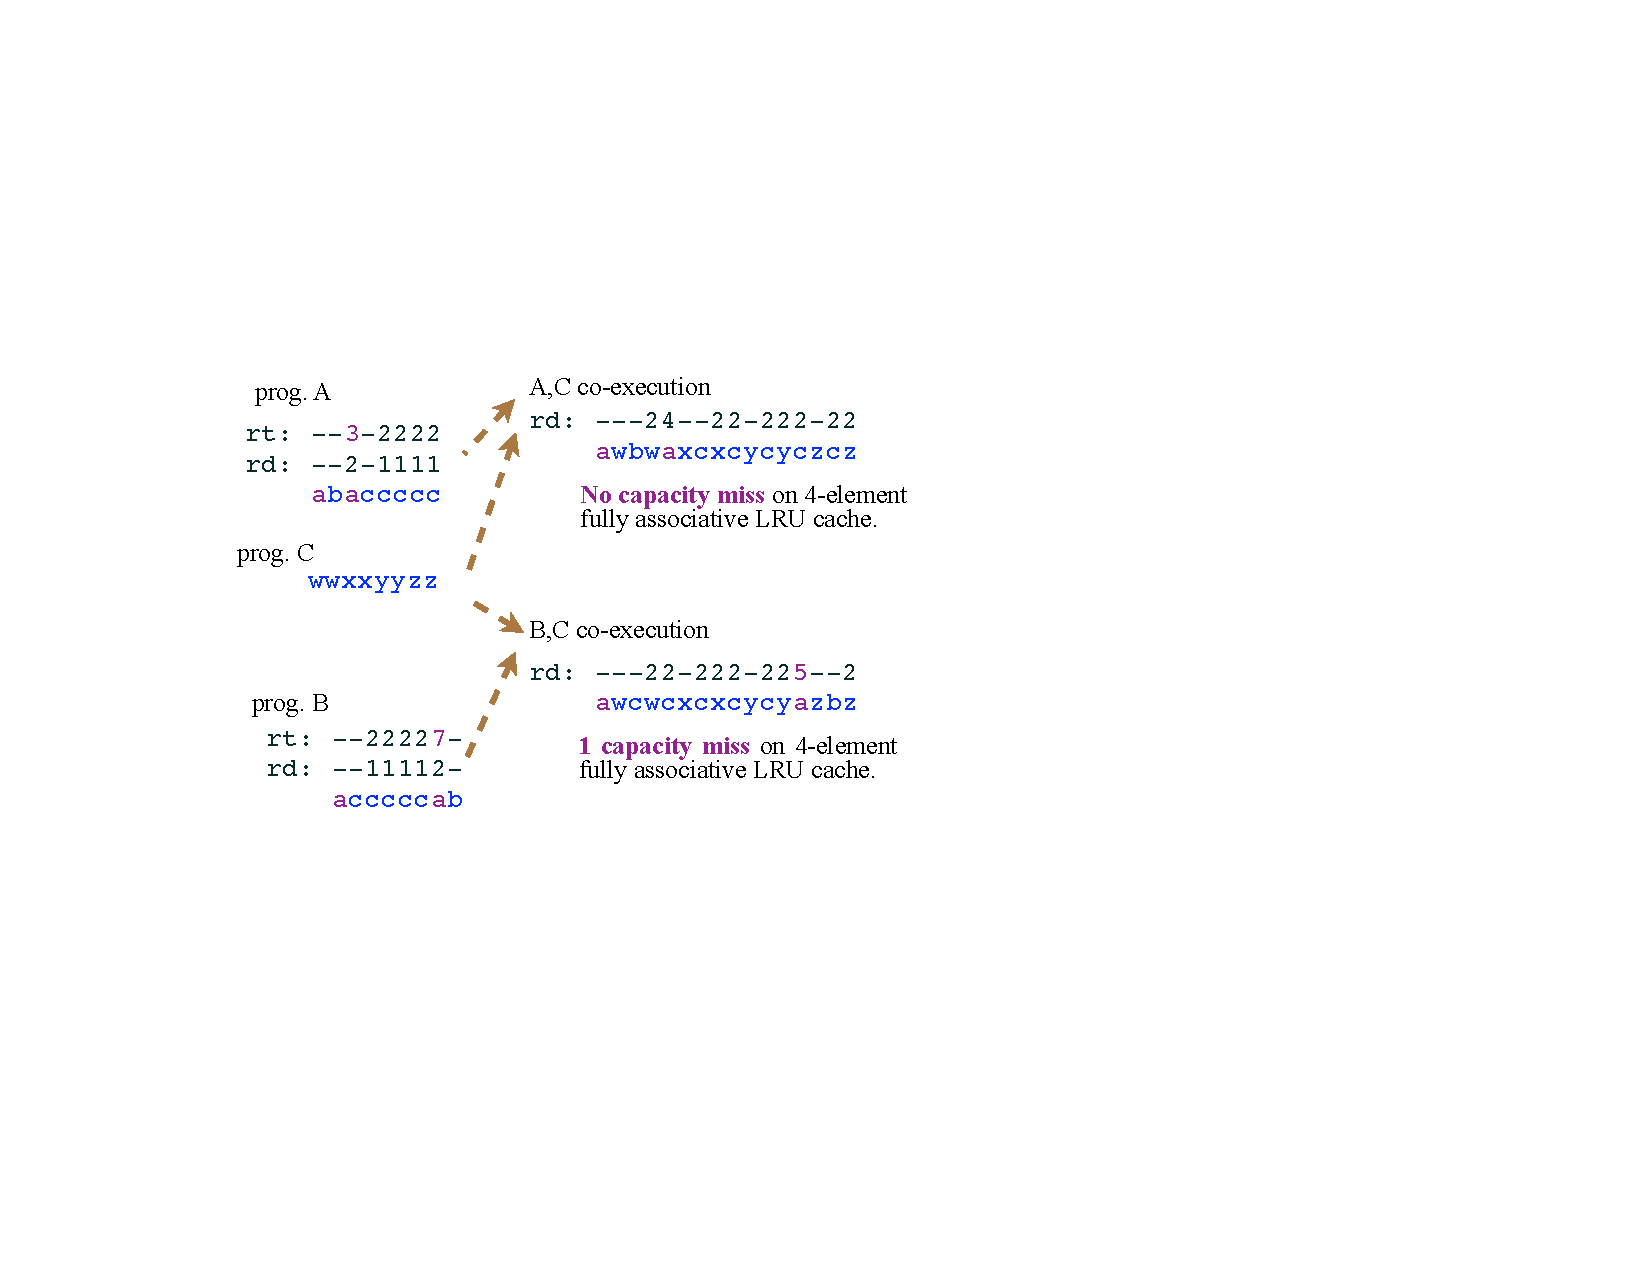
\includegraphics[width=11cm]{figures/intro/rdft_comp}
\label{intro_rdft_comp}
\caption{Programs $A,B$ have the same reuse distances ('-' means $infty$) and hence capacity miss
  ratio. $A,C$ co-run incurs no capacity miss in shared cache, but
  $B,C$ co-run does.  The difference is caused not by the footprint.}
\end{figure}

The reason is the different interaction based on the time span of 
a reuse.  Consider the data accesses to $a$ in $A,B$.  They
have the same private reuse distance, $2$, but very different
(logical) reuse times, $3$ in $A$ and $7$ in $B$.  When co-running with
$C$, the reuse distance is lengthened because of the data accesses by
$C$.  Since the reuse in $B$ spans over a longer time, it is affected
more by cache sharing.  As a result, the concurrent reuse distance for
$a$ is 4 in the $A,C$ but 5 in the $B,C$ co-run.

\citet{Chandra+:HPCA05} described three models of cache sharing.  A
simple one is the composition of reuse distance, called \emph{ (LRU)
  stack distance competition} (SDC).  Since the model uses the reuse
distance as the only input, it would have given the same prediction in
our example for $A,C$ and $B,C$.  Therefore, it is a flawed model.  A
number of earlier studies have found the same conclusion through
experiments \citep{Fedorova+:CACM10,Zhuravlev+:ASPLOS10,Blagodurov+:TOCS10}.

\subsection{The Classic Composition Model}
\label{sec:back:classic}

Let $A,B$ be two programs share the same cache but do not shared data,
the effect of $B$ on the locality of $A$ is:

\begin{eqnarray*}
P(\mbox{capacity miss by A when running with B}) \\
= P(\mbox{ A's reuse distance + B's footprint $\ge$ cache size})
\end{eqnarray*}

In this model, the cache interference (i.e. CRD) is computed by
combining the footprint, i.e. the interference, and the reuse
distance, i.e. the per-task locality.  Specialized versions of
this model is first developed by \citet{Suh+:ICS01} for time-sharing
systems and \citet{Chandra+:HPCA05} for multicore cache sharing.  
While \citet{Chandra+:HPCA05} described and evaluated the composition
for two programs, \citet{ChenA:HPCA09} improved the accuracy when
analyzing more programs with a greater number of cache conflicts.
A later study by \citet{Jiang+:HiPEAC10} gave the general form of
the classic model not tied to cache parameters such as associativity.  

In \citet{Suh+:ICS01} and \citet{Chandra+:HPCA05}, the footprint
equation is iterative
(see Section~\ref{sec:back:fp}).  In \citet{Jiang+:HiPEAC10}, 
the footprint equation is statistical (see Section~\ref{sec:back:rd}).
Another footprint equation is the
conversion formula by \citet{DenningS:CACM72}.
These equations are not completely constrained, so the solution
is not unique and depends on modeling assumptions.  

The classic model is not simple as presented in the previous
publications.  In \citet{Chandra+:HPCA05}, hardware and program
factors were considered together.  \citet{XieL:MSI08} noted that the
model by Chandra et al. ``is fairly involved; the large number of
complex statistical computations would be very difficult to directly
implement in hardware.''  In addition, the model has a high cost.  It
was not used in the comparison study of \citet{Zhuravlev+:ASPLOS10},
because it was not ``computationally fast enough to be used in the
robust scheduling algorithm.''  

There is another weakness in usability.  The two inputs, reuse distance and
footprint, do not have a simple effect on the composed output.  The
complexity hinders the use of composable model in practice.  As introduced in
Section~\ref{sec:intro:theory}, the new locality theory will derive
the classic model as a special case.  The theory defines the footprint
as a type of all-window statistics that have precise and real-time
solutions.  It gives a host of other composition methods for easier use
in performance analysis.


\section{Performance Models of Shared Cache}

% measurement, characterization, prediction, optimization

Direct measurements, either by testing or simulation, is often
necessary to identify hardware and timing dependent effects.

\subsection{Performance Monitoring and Analysis}

Performance analysis for parallel code has a long history \citep{Meira+:Carnival96,Reed+:ICPPW96,Darema+:Metrics87}.
Modern processors provide hardware counters to monitor hardware events
with little or no run-time cost.  The events related to memory
performance include the frequency of cache misses, cache coherence
misses, and various cycle counts including stalled cycles.  
When many events are being monitored in a large system over a long
execution, the large volume of results presents two problems.  The
first is the time and space cost of collecting and storing these
results.  The second is analysis---how to identify high-level
information from low-level measurements.  

These problems are solved by monitoring and visualization tools
including commercial ones such as Intel VTune Amplifier, AMD
CodeAnalysist, and CrayPat, and open-source projects such as PAPI
library \citep{Browne+:JHPCA00}, HPCToolkit \citep{Adhianto+:CCPE10},
TAU \citep{ShendeM:IJHPCA06}, and Open$|$SpeedShop
\citep{Schulz+:SP08}.  The aggregation of information is usually code
centric, which shows performance in program functions and
instructions.  Vertical profiling identifies performance problems
across a software stack \citep{Hauswirth+:SPE10}.  Continuous program
optimization (CPO) not just finds performance problems but also
optimizes performance
automatically \citep{Cascaval+:PACT05,Tam+:ASPLOS09,Childers+:IPDPS03,Cascaval+:JRD06}.  In recent work,
data-centric aggregation is used to pin-point locality problems more
effectively, for issues of not just cache misses but also non-uniform
memory access (NUMA) latency
\citep{McCurdyV:ISPASS10,LiuM:CGO11,LiuM:PPOPP14}.


% Memphis 

% Kale+:FGCS06

\subsection{Optimal Co-scheduling}

% Need exhaustive testing.  SDC is not a valid model since reuse
% distance is not composable.

Given a set of programs, co-scheduling is to divide them into co-run
groups, where each group is run together.  The goal is to minimize the
interference within these groups, so to maximize resource utilization
and co-run throughput.  The interference depends mostly on the
memory hierarhcy, and the effect is non-linear and
asymmetric.  

While a locality model may predict the cache interference, the impact
on performance depends on many other factors including the CPU speed,
the effect of prefetching, the available memory bandwidth, and if a
program is I/O intensive, the speed of the disk or the network.
Direct testing can most accurately measure the performance
interference.  Complete testing, however, has an exponential cost
since the number of subsets in an $n$-element set is $2^n$.
Note that solo executions are needed so to compute the slowdown
in group executions.

For pairwise co-runs, the interference can be represented by a
complete graph where nodes are programs and edges have weights equal to
pair-run slowdowns. \citet{Jiang+:TPDS11}\footnote{first published in
  \citet{Jiang+:PACT08}.} showed that the optimization is min-weight
perfect matching, and the problem is NP-hard.  They gave an
approximation algorithm that produces near-optimal schedules.

The throughput is often not the only goal.  Other desirable properties
include fairness, i.e. no program is penalized disproportionally due
to unfair sharing, and quality of service (QoS), i.e. a program must
maintain a certain level of performance.

As inputs, an optimal solution requires accurate prediction of co-run
degradation.  Prior solutions are either locality based (see
Section~\ref{sec:locality:sharing}) or performance based (this
section).  It is difficult for them to produce accurate prediction
without expensive testing.  For co-run miss rates, the new footprint
theory enables near real-time prediction, with an accuracy similar
to exhaustive testing (see Section~\ref{sec:iter-rank}).

\subsection{Characterization of Interference}

\citet{XieL:MSI08} gave an animalistic classification of program
interference.  Based on the behavior in shared cache, a program
belongs to one of the four animal classes.  A turtle has little use of
shared cache.  A rabbit and a sheep both have a low miss rate.  A
rabbit is sensitive and tends to be affected by co-run peers, but a
sheep does not.  Both programs have small impacts on others.  The last
class is devil, which has a high miss rate, impairs the performance of
others, but is not affected by others.  

Other classifications include coloring of miss intensity, dual metrics
of cache partitioning, and utility of cache space to performance.
These are reviewed in \citet{XieL:MSI08}.

\citet{Jiang+:HiPEAC10} classified programs along two locality
dimensions.  The \emph{sensitivity} is computed from the classic
composition model (Section~\ref{sec:back:classic}).  It shows how a
program is affected by others, The \emph{competitiveness} is distinct
data blocks per cycle (DPC), which is equivalent to the average
footprint.  If we divide each locality dimension into two halves, we
have four classes, which may call \emph{locality classes}.  Locality
classes are not the same as animal classes.  For example, a program
can be extremely competitive, i.e.  devilish, but may be either
sensitive or insensitive.  The phenomenon is observed by
\citet{Zhuravlev+:ASPLOS10}, who showed that the animalistic
classification is incomplete because ``devils were some of the most
sensitive applications.''  

The experimental data in this thesis also confirms the locality model
and will show that the program behavior in shared cache is
characterized by the two dimensions given by \citet{Jiang+:HiPEAC10}.
In Chapter~\ref{chap:model}, these two dimensions are called
shared-cache \emph{sensitivity} and \emph{pressure}.  

% However, the evaluation in this work will be based on the miss rate,
% not execution time.

\subsection{Predictive Performance Models}

In symbiotic scheduling (SOS), \citet{SnavelyT:ASPLOS00} used a
sampling phase to test a number of possible co-run schedules and
select the best one from these samples for the next (symbiosis) phase.
They showed that a small number of possible schedules (instead of
exhaustive testing) is sufficient to produce good improvements.  The
system was designed and tested for simultaneous multi-threading.
Symbiotic scheduling assumes that program co-run behavior does not vary
significantly over time, so the sampling phase is representative of
performance in the remaining execution.  Testing does not require
program instrumentation.

% read the papers VaswaniZ:SOSP91 and related on memory locality
% scheduling

\citet{Fedorova+:PACT07} addressed the problem of performance
isolation by suspending a program execution when needed.  They gave a
cache-fair algorithm to ensure a program runs at least at the speed
with fair cache allocation.  The technique is based on the assumption
that if two programs have the same frequency of cache misses, they
have the same amount of data in cache.  In locality modeling, the
assumption means uniform distribution of the access in cache.  While
the assumption is not always valid, the model is efficient for use in
an OS scheduler to manage cache sharing in real time.

The two techniques are dynamic and do not need off-line profiling.
However, on-line analysis may not be accurate and cannot predict
interference in other program combinations. Furthermore, non-symbiotic
pairing (during sampling) and throttling (for fairness) do not
maximize the throughput.

%Cache-fair scheduling protects fairness but does not maximize CPU
% utilization since not all programs are run at all times.

\citet{Blagodurov+:TOCS10}\footnote{Journal version of
  \citep{Zhuravlev+:ASPLOS10,Fedorova+:CACM10}.} developed \emph{Pain}
classification.  The degree of pain that application A suffers while
it co-runs with B is affected by A's cache sensitivity, which is
computed using the reuse distance profile (PRD), and B's cache
intensity, which is measured by the number of last level cache
accesses per million instructions.  The Pain model is similar to the
classic composition model described in Section~\ref{sec:back:classic}
except that Pain uses the miss frequency rather than the footprint.
The choice is partly for efficiency.  Other online techniques also use
the last-level cache miss rate as cache use intensity
\citep{Shen:ASPLOS10,knauerhase2008micro}. 

Pain is an offline solution.  The idea is extended into an online
solution called Distributed Intensity (DI), which uses only the miss
rate.  An application is classified as intensive if it is above the
average miss rate and nonintensive otherwise.  The scheduler then
tries to group high-resource-intensity program(s) with
low--resource-intensity program(s) on a multicore to mitigate the
conflicts on shared resources \citep{Blagodurov+:TOCS10,Zhuravlev+:ASPLOS10,Fedorova+:CACM10}.

Cache misses represent only a (small) subset of program accesses.  In
comparison, the footprint includes the effect of all cache accesses.
Furthermore, the miss frequency depends on co-run peers and has the
effect of circular feedback since the peers are affected by self.  The
result of counter-based modeling is specific to one grouping situation
and may not be usable in other groupings.  In comparison, footprint
analysis collects ``clean-room'' statistics, unaffected by co-run
peers program instrumentation or the analyzer code
and usable for interference with any peers (which may be
unknown at the time of footprint analysis).  With the new theory in
this thesis, footprint can be obtained with near real-time efficiency.

% proportional to the expectation of its reuse distance distribution

In an offline solution, \citet{Jiang+:TPDS11} defined the concept of
\emph{politeness} for a program as ``the reciprocal of the sum of the
degradations of all co-run groups that include the job.''  The
politeness is measured by the effect on the execution time, not just
the miss ratio, and is used to approximate optimal job scheduling.

In an online solution, the high cost of co-run testing is addressed in
a strategy called Bubble-Up~\citep{Mars+:IEEEM12}.  The strategy has
two steps.  First, a program is co-run against an expanding bubble to
produce a sensitivity curve.  The bubble is a specially designed probe
program.  In the second step, the pressure of the program is reported
by another probe and probing run.  Bubble-Up is a composable strategy
since each program is tested individually without testing all program
combinations.  The Bubble-Up pressure and sensitivity are factors of a
program's run-time.  In Chapter~\ref{chap:model}, we define cache
pressure and sensitivity are factors of the program's behavior in
shared cache. 

% The time factors are useful for task scheduling, while the cache
% factors for program locality optimization.

Two recent solutions used machine learning.
\citet{DelimitrouK:ASPLOS13} built a data center scheduler called
Paragon.  The design of Paragon identifies 10 sources of interference.
It uses offline training (through probe programs) to build
parameterized models on their performance impact.  During online use,
Paragon feeds the history information to a learning algorithm called
collaborative filtering.  Collaborative filtering supports sparse
learning.  Based on a small number of past data, it can predict
application-application interference and application-machine match.

\citet{Zhao+:PACT13} developed a model of pressure that includes both
cache and memory bandwidth sharing.  The model is not peer specific.
The same pressure may be caused by one program or a group of programs.
The model is built using regression analysis.  

Statistical techniques have had many uses in performance analysis of
parallel code, including clustering, factoring and correlation
\citep{AhnV:SC02}, linear models (with non-linear
components) \citep{Rodriguez+:EuroPar04}, queuing
models \citep{Jacquet+:IPDPS03}, directed
searches \citep{Miller+:Computer95}, and analytical models
\citep{Kerbyson+:IPS03}.

Machine learning is general and can consider different types of
resources together.  It is also scalable as more factors can be added
by having additional learning.  In comparison, this thesis aims not to
generalize but to specialize, with the sole focus on locality and cache
sharing.  It develops mathematically tractable models that can derive
co-run results.  In comparison, Paragon's learning technique observes
the co-run results but has to be given the solo-run speed to compute
the co-run slowdown.  The cache model complements performance models,
which can include the specialized model as a component.  Locality
metrics such as the footprint can be used as an input to a learning
algorithm.

% theoretically sound, empirically accurate (for miss rate prediction)

% need to know the solo run speed.

Using the PRD/CRD model \citep{WuY:PACT11}, \citet{Wu+:ISCA13}
conducted experiments on a wide range of symmetric multithreaded
benchmarks on modest problem size and core counts and used their
scaling framework to study the performance (average memory access time
AMAT) over cache hierarchy scaling for large problem sizes on
large-scale (LCMP)s.  The study focused on the effect of hardware
characteristics such as core counts, cache sizes and cache
organizations on different programs and program inputs, but not
hardware independent program characterization.


\section{Other Techniques}

\paragraph{Cross-run inference}

As a measure of locality, reuse distance is not tied to particular
code path, data address, or code layout.  It has been used to compare
the locality between different executions to identify cross-run
characteristics.  Earlier work includes whole-program
locality \citep{Zhong+:TOPLAS09,DingZ:PLDI03,Shen+:LACSI03}, 
cross-architecture performance
prediction \citep{MarinM:SIGMETRICS04,MarinM:LACSI05},
miss-rate prediction across inputs \citep{Zhong+:TOC07},
and locality phases \citep{ShenD:LCPC05,Shen+:ASPLOS04,Shen+:JPDC07}.

More recently, a series work shows how to predict the loop trip count
using cross-run learning.  A number of learning techniques such as 
classification trees have been used \citep{CavazosM:PLDI04,MaoS:CGO09}.
\citet{MaoS:CGO09} defined an extensible 
input characterization language (XICL).  One application 
of input-centric learning is to improve the JIT optimization in Java
JVM \citep{Arnold+:OOPSLA05,Tian+:OOPSLA10,Tian+:OOPSLA11}.
Another type of behavior correlation is between
different loop trip counts within an execution and between different
types of values.  \citet{Jiang+:CGO10} could automatically identify
a small set of values that can predict the overall program behavior.
\citet{Wu+:OOPSLA12} expanded the correlation analysis to include
sequence patterns.  

Profiles from different inputs are routinely used in feedback-driven
program optimization (FDO) and iterative compiler optimization.
The effect of compiler optimization depends on the quality of profiles.  The
dependence has been examined using statistics \citep{Chen+:PLDI10,Wu+:ECOOP13}.

\paragraph{Bursty Sampling}
Arnold and Ryder pioneered a general framework to sample Java code,
i.e. the first few invocations of a function or the beginning iterations of a
loop~\citep{ArnoldR:PLDI01}.  It has been adopted for hot-stream
prefetching in C/C++ in bursty sampling~\citep{ChilimbiH:PLDI02} and
extended to sample both static and dynamic bursts for calling context
profiling~\citep{Zhuang+:PLDI06}.  Shadow profiling pauses a program at
preset intervals and forks a separate process to profile in parallel
with the base program~\citep{Moseley+:CGO07,WallaceH:CGO07}. The 
reuse distance analysis is not a good target for these techniques because
of the uncertain length of the reuse windows.  However, we will
show that the footprint is easily measured using shadow profiling.
Reuse distance can then be computed using the conversion theory.

% cite Bond

\paragraph{Trace compression} To profile all-window footprint
efficiently without window sampling, trace compression is introduced
into this context. 
Kaplan et al. studied the problem of optimal trace compression to generate the
shortest possible trace that still preserves same LRU behavior in
large cache~\citep{Kaplan+:TOMACS03}. Two algorithms, {\em Safety
  Allowed Drop(SAD)} and {\em Optimal LRU Reduction(OLR)}, were
proposed. $SAD$ compressed the trace by removing references which
affect the order that data was fetched 
into or evicted from an $LRU$(or $OPT$) memory. The guideline for 
reference removing was stated as: for any three references 
to the same page in a trace, if the LRU distance between the first and
third reference is less than k, then removing the middle reference 
does not affect the outcome of $LRU$ and $OPT$ simulation on memories 
of size no greater than k ~\citep{Kaplan+:TOMACS03}.

Despite significant amount of references removed from actual traces 
by $SAD$, it does not guarantee to give optimal(shortest) reduced 
trace for $LRU$ and $OPT$ simulation. Instead of removing
useless references for simulation purpose, $OLR$ is proposed to 
achieve the optimal reduced trace. $OLR$ solved the problem from 
an opposite direction. $OLR$ scans the input trace, tags each references,
and then keeps the references that are necessary for $LRU$ or 
$OPT$ simulation.

One of our footprint algorithms, which will be introduced in
Chapter~\ref{chap:fp},  uses similar trace compression.
Both techniques use intervals as the basic unit in analysis 
and ignore the references that do not effect the analysis result.


% The miss count is measured in real time to be hardware specific and
% peer dependent.



\begin{comment}
Current performance models focus on parallelism, memory demand, and
communication pattern.  The prevalence of two-level parallelism on
multicore systems is widely recognized.  A recent example is Singh et
al., who characterized a multicore machine as an SMP of CMPs and
showed the importance of modeling the two levels in predicting the
performance and scalability in multithreaded HPC
applications~\citep{Singh+:EuroPar10}.  In their study, the cache
performance was measured by counting the L1 cache misses.  Sancho et
al. evaluated the performance impact on large-scale code from shared
and exclusive use of memory controllers and memory
channels~\citep{Sancho+:LSPP10}.  A fundamental limitation in
performance scaling is memory bandwidth, which depends on how programs
share cache on a CMP.  Hao et al. proposed a novel processor design
that used data migration in shared L2 cache to mitigate the NUMA
effect~\citep{Hao+:HPCC08}.  Cache migration, although reduces latency,
does not directly change the bandwidth demand of a group of tasks.

Most HPC performance tools gather hardware counter results.  An
example is Open$|$SpeedShop, which provides a real-time display while
an MPI program is running~\citep{Schulz+:SP08}.  The emphasis is
measurement rather than prediction.  HPCView uses a collection of
program metrics including the reuse distance and can predict cache
performance for different cache sizes and configurations but does not
predict the effect of cache sharing~\citep{MC+:JS02}.  HPCToolkit can
analyze optimized parallel code with only a few percent
overhead~\citep{Adhianto+:CCPE10}.  To control the cost, HPCToolkit
does not instrument program data access.

The time sharing system is the first co-run environment.  There
programs time share the processor and do not actually run at the same
time.  Cache sharing models were invented by the studies on the effect
of time sharing in cache.  In particular, Thiebaut and
Stone~\citeyear{ThiebautS:TOCS87} and Suh et al.~\citeyear{Suh+:ICS01}
computed the cache interference by the impact of the peer footprint on
the self locality.  Thiebaut and Stone coined the term \emph{cache
  footprint}.  The cache footprint is for a single window size, the
length of the time quanta.  

Chandra et al.~\citeyear{Chandra+:HPCA05} is the first to use such
model in a multicore environment where programs co-run continuously.
They had to solve the footprint problem for all window sizes, for which
they use statistical solutions (see Section~\ref{sec:fp-measure}) and show accurate miss ratio prediction.

Cache sharing in multi-threaded code is affected by two additional
factors: data sharing and thread interleaving.  The effect can be
characterized by extending the concept of reuse
distance~\citep{Schuff+:PACT10,Schulz+:CF05} or inferred using a
composable model~\citep{DingC:MSR09,Jiang+:CC10}. 

According to the extended definition~\citep{Schuff+:PACT10}, the reuse
distance of a reference is infinite if the reference accesses an
address that has not been accessed before or that has been overwritten
by other threads;  Otherwise, the reuse distance is the number of
distinct data accessed by all threads which shared memory with current
thread within the reuse window. Shared reuse buffer was used to
measure this  extended reuse distance. Experiments validated the
success of  introducing multicore-awareness to locality analysis. The
accuracy of locality-based miss ratio prediction was improved by 70\%
for per-core cache and 90\% for shared caches on average of several
OpenMP and transaction-based benchmarks. 

The compositional model ~\citep{DingC:MSR09}, used an iterative method
and a sampling method to estimate all-window footprint. The sampling
rate was O(1=N), and there was no guarantee in the result. 

The miss rate curve has been used for memory partitioning to ensure
fairness or maximize throughput in a parallel
workload~\citep{Zhou+:ASPLOS04}.  Similarly, reuse distance has been
used for cache partitioning among data
objects~\citep{Lu+:PACT09}. Recently, Zhuravlev et al. reviewed four
models based on the miss rate and the reuse
distance~\citep{Zhuravlev+:ASPLOS10}.  As on-line models, these
techniques did not consider the working set metrics because of the
cost.  For example, Zhuravlev et al. considered a less accurate model
from Chandra et al. because for efficiency it did not require all-window footprints~\citep{Chandra+:HPCA05}.  Zhuravlev et al. showed that cache sharing is one
of the factors but not necessarily the major factor~\citep{Zhuravlev+:ASPLOS10}.
Still, an accurate and fast solution may help to quantify the
contribution from cache sharing in the overall interference.

Chandra et al. also gave a model that used only the reuse
distance~\citep{Chandra+:HPCA05}.  Zhuravlev et al. used it and two
other such models and found that in task scheduling, they did not
significantly outperform a simple model that used only the miss
rate~\citep{Zhuravlev+:ASPLOS10}.

Cache sharing is only one factor in performance.  Others include the
sharing of memory interface and the CPU
scheduler~\citep{Zhuravlev+:ASPLOS10}.

To estimate the fair allocation, the paper uses the balls
and bins model, where cache is a bin, and different programs throw
different color balls into the cache upon misses.  Assuming a uniform
distribution in cache access, co-run programs with the same miss rate
would have the same amount of data in cache, hence a fair allocation.
\citet{Fedorova+:PACT07} developed a highly efficient scheduler
and showed strong performance isolation on a range of benchmark
programs.  

Since the Pain model is based on
reuse distance only so it has the limitation described in
Section~\ref{sec:rd:limit}.  In practice, however, it could achieve
performance close to the best possible
\citep{Blagodurov+:TOCS10,Zhuravlev+:ASPLOS10,Fedorova+:CACM10}.

\subsection{Program co-scheduling}

Since online scheduling requires low overhead, existing approaches utilize hardware 
event counters, which can be read at little cost.  

Pain is a composable model.  It differs from paw in the notion of
cache intensity.  It is defined using a single window size.  In
computing B's interference of A, $all-footprint analysis$ considers
all window sizes in B since a reuse window in A may have an arbitrary
length.

For instance, a program may incur substantially more cache misses
after the peers change because its share of cache space in the new
grouping becomes too small for its working set.  In contrast, the
lifetime sampling approach in this paper properly models the cache
sharing in all (hypothetical) program grouping situations.  

\subsection{Shared Cache Optimization and Scheduling}

QoS-Compile from Tang et al.~\citep{Tang+:CGO12} is a compiler solution
to mitigate memory hierarchy contention for independent co-run
programs. The optimization first requires a profiling pass to identify
contentious code regions.  % ASPLOS

The miss count has been used to model the cache
fairness~\citep{Fedorova+:PACT07}.  The model assumes that the cache
access is uniformly distributed.  The miss count is measured in real
time to be hardware specific and peer dependent.  The requirements of
QoS compile, fairness and optimal scheduling are opposite to the needs
of offline program optimization, for which the metrics should be
hardware and peer independent.

\paragraph{Program Tuning Tools}
Continuous program
optimization (CPO) uses the special support in an experimental IBM
system to mark exact data addresses~\citep{Cascaval+:PACT05}.
Subsequent accesses to marked data are trapped by hardware and
reported to software.  Similar hardware support has been used to
predict the miss-rate curve~\citep{Tam+:ASPLOS09} and quantify
data locality~\citep{LiuM:CGO11}.   Hardware sampling, however,
is necessarily sparse or short in order to be efficient.  StatCache and CPO use a
small number of samples.   HPCToolkit is constrained by the hardware
limit of 64K events on the AMD machine~\citep{LiuM:CGO11}.  
Lifetime sampling is based on the locality theory described in Section~\ref{sec:back}.
It instruments and
collects the data access trace as long as needed based on the cache
lifetime.  The current implementation is entirely software, which is
portable.  Lifetime sampling may take advantage of special
hardware and OS support if they are available.

A similar algorithm may be used to collect other types of all-window statistics
such as all-window miss rates or all-window thread
interleaving~\citep{DingC:PPOPP08}.

Time-based conversion is used
in reuse distance profiling~\citep{Shen+:POPL07} and recently modeling
cache sharing~\citep{Eklov+:HiPEAC11,EklovH:ISPASS10}.
Another approach, more efficient but not entirely data driven, is to
assume common properties in data access and distinguish
programs through parameter
fitting~\citep{IbrahimS:ICPP10,He+:IPDPS12}.


\end{comment}

